\documentclass{beamer}
%\documentclass[handout]{beamer}

% https://www.overleaf.com/learn/latex/Beamer_Presentations:_A_Tutorial_for_Beginners_(Part_2)%E2%80%94Lists,_Columns,_Pictures,_Descriptions_and_Tables
\usepackage{amsmath}
\usepackage{amsfonts}
\usepackage{amssymb}

\usepackage{tabularx,tabulary,longtable}
\newcolumntype{Z}{>{\raggedleft\arraybackslash}X}
\newcolumntype{Y}{>{\centering\arraybackslash}X}

\usepackage[utf8]{inputenc}
%\usepackage{helvet}

\usetheme{Madrid}
\useinnertheme{rectangles}



%Information to be included in the title page:
\title{LAW 3: Examples}
\date{\today}


\author[Dr Ian Hunt] % (optional, for multiple authors)
{Dr Ian Hunt\inst{1}}

\institute[Monash University] % (optional)
{
	\inst{1}%
	Manager, Statistical Consulting Service\\Data Science and AI Platform\\
	Monash University\\
	ihunt@bunhill.co.uk; ian.hunt@monash.edu; statisticalconsulting@monash.edu
}



\usepackage[T1]{fontenc} % displays speacial 
\usepackage{graphicx,psfrag,epsf}
\usepackage{pdfpages}

\usepackage{url} % not crucial - just used below for the URL 


\makeatletter
\newcommand*{\centerfloat}{%
	\parindent \z@
	\leftskip \z@ \@plus 1fil \@minus \textwidth
	\rightskip\leftskip
	\parfillskip \z@skip}
\makeatother


%\usepackage[compatibility=false]{caption}
\usepackage{graphicx}

\usepackage{tabularx,tabulary,longtable}
\usepackage{booktabs}

%
\usepackage{enumerate}
%\usepackage{enumitem}
%\usepackage{enumitem}
\usepackage{setspace}



\usepackage{natbib}
\usepackage{bibentry}
\makeatletter 
\renewcommand\BR@b@bibitem[2][]{\BR@bibitem[#1]{#2}\BR@c@bibitem{#2}}        
\makeatother
%\nobibliography*
\nobibliography{data/ianBIBmaster.bib}
\bibliographystyle{Chicago}

\AtBeginSection[]
{
	\begin{frame}
		\frametitle{Table of Contents}
		\tableofcontents[currentsection]
	\end{frame}
}



\newcommand{\littlePIC}{.35\textwidth}
\newcommand\jc[1]{{\itshape #1}}

%\theoremstyle{theorem}
%\newtheorem*{maths}{\translate{Maths}}

\theoremstyle{example}
\newtheorem*{maths}{\translate{Maths}}

\usepackage{caption}
\setbeamertemplate{caption}[numbered] 
%\captionsetup{font=scriptsize,labelfont=scriptsize}
\setbeamerfont{caption}{size=\scriptsize}




\newenvironment{bigitemize}{\itemize\addtolength{\itemsep}{1em}}{\enditemize}
\newenvironment{bigenumerate}{\enumerate\addtolength{\itemsep}{1em}}{\endenumerate}


\newcommand{\outcomes}{	The broad goals are to enable you to do empirical research on a computer and ensure that you are not anxious about ``stats packages'' or computing languages.
	\\~\\
	\begin{bigenumerate}
		\item<+-> Understand the basics of ``statistical computing''.
		\item<+-> Select the right software or language for your research and data.
		\item<+-> Avoid time-wasting, needless complexity and dirty habits.
		\item<+-> Recognise some good ideas.
	\end{bigenumerate}
}

\begin{document}
	
	
	\frame{\titlepage}
	
	\begin{frame}
		\tableofcontents[hideallsubsections]
	\end{frame}
	
	
	\begin{frame}{Lecture outcomes}
		\outcomes
	\end{frame}
	
	
	
	
	\begin{frame}{With the data comes a ``minimal model''}
		A minimal model is one that allows you structure the data into a matrix.\\~\\
		\begin{bigitemize}
			\item<+-> The matrix has \emph{rows} and \emph{columns}.
			
			\item<+-> The \textbf{rows} represent meaningful units e.g.\ law cases, patients, survey participants.
			
			\item <+-> The \textbf{columns} represent information about or from each unit e.g.\ case length, patient age, survey responses.
			
			\item<+-> Much of what passes for ``data science'' is about the efficient structuring and manipulation of this sort of minimal model.
			
		\end{bigitemize}
	\end{frame}
	
	
	\begin{frame}{Summarizing the ``minimal model'' --- its estimation}
		Basic parameter estimation is essential.\\~\\
		\begin{bigitemize}
			\item<+-> Summary statistics  and charts \textbf{down columns}: mean, variance, standard deviations, min/max, quantiles, histograms etc.
			
			\item<+-> Summary statistics and charts \textbf{across columns}: measures of correlation; scatter plots; boxplots.
			
			\item<+-> Lumping rows into meaningful \textbf{groups} via categories: male/not-male; NSW/Vic; treatment/placebo; old/young and so on.
			
			\item<+-> Comparing summary statistics \textbf{between row groups} (and using contingency tables for counts): means for males/non-males; mean settlement in NSW/Vic cases; death rates of treatment/placebo; and so on.
			
		\end{bigitemize}
	\end{frame}
	
	
	%\begin{frame}{Example}
	%table of summary stats
	%
	%table of summary stats by group
	%
	%come charts (!)
	%
	%a contingency table
	%\end{frame}
	
	
	
	\begin{frame}{Comparing summaries is ``model assessment''}
		\begin{bigitemize}
			\item<+-> Line up charts by eye!
			\item<+-> Use t-tests for comparison of means.
			\item<+-> Compare confidence intervals between groups and relative to meaningful benchmarks.
			\item<+-> Consider \textbf{transforming} for robustness to the influence of outliers.
			\begin{itemize}
				\item For example to turning skewed counts into ranks or take their logs.
			\end{itemize}
			\item<+-> Use chi-squared tests to hunt for differences between groups within contingency tables.
		\end{bigitemize}
		
		\onslide<+->
		\textbf{Rinse and then repeat ...}
		
	\end{frame}
	
	
	\begin{frame}{Lets do an iteration ... }
		
		\centerfloat \centering	
		\includegraphics[width=.95\textwidth]{data/data-detective1.pdf}
		
	\end{frame}
	
	\begin{frame}{On this data}
		\centerfloat \centering	
		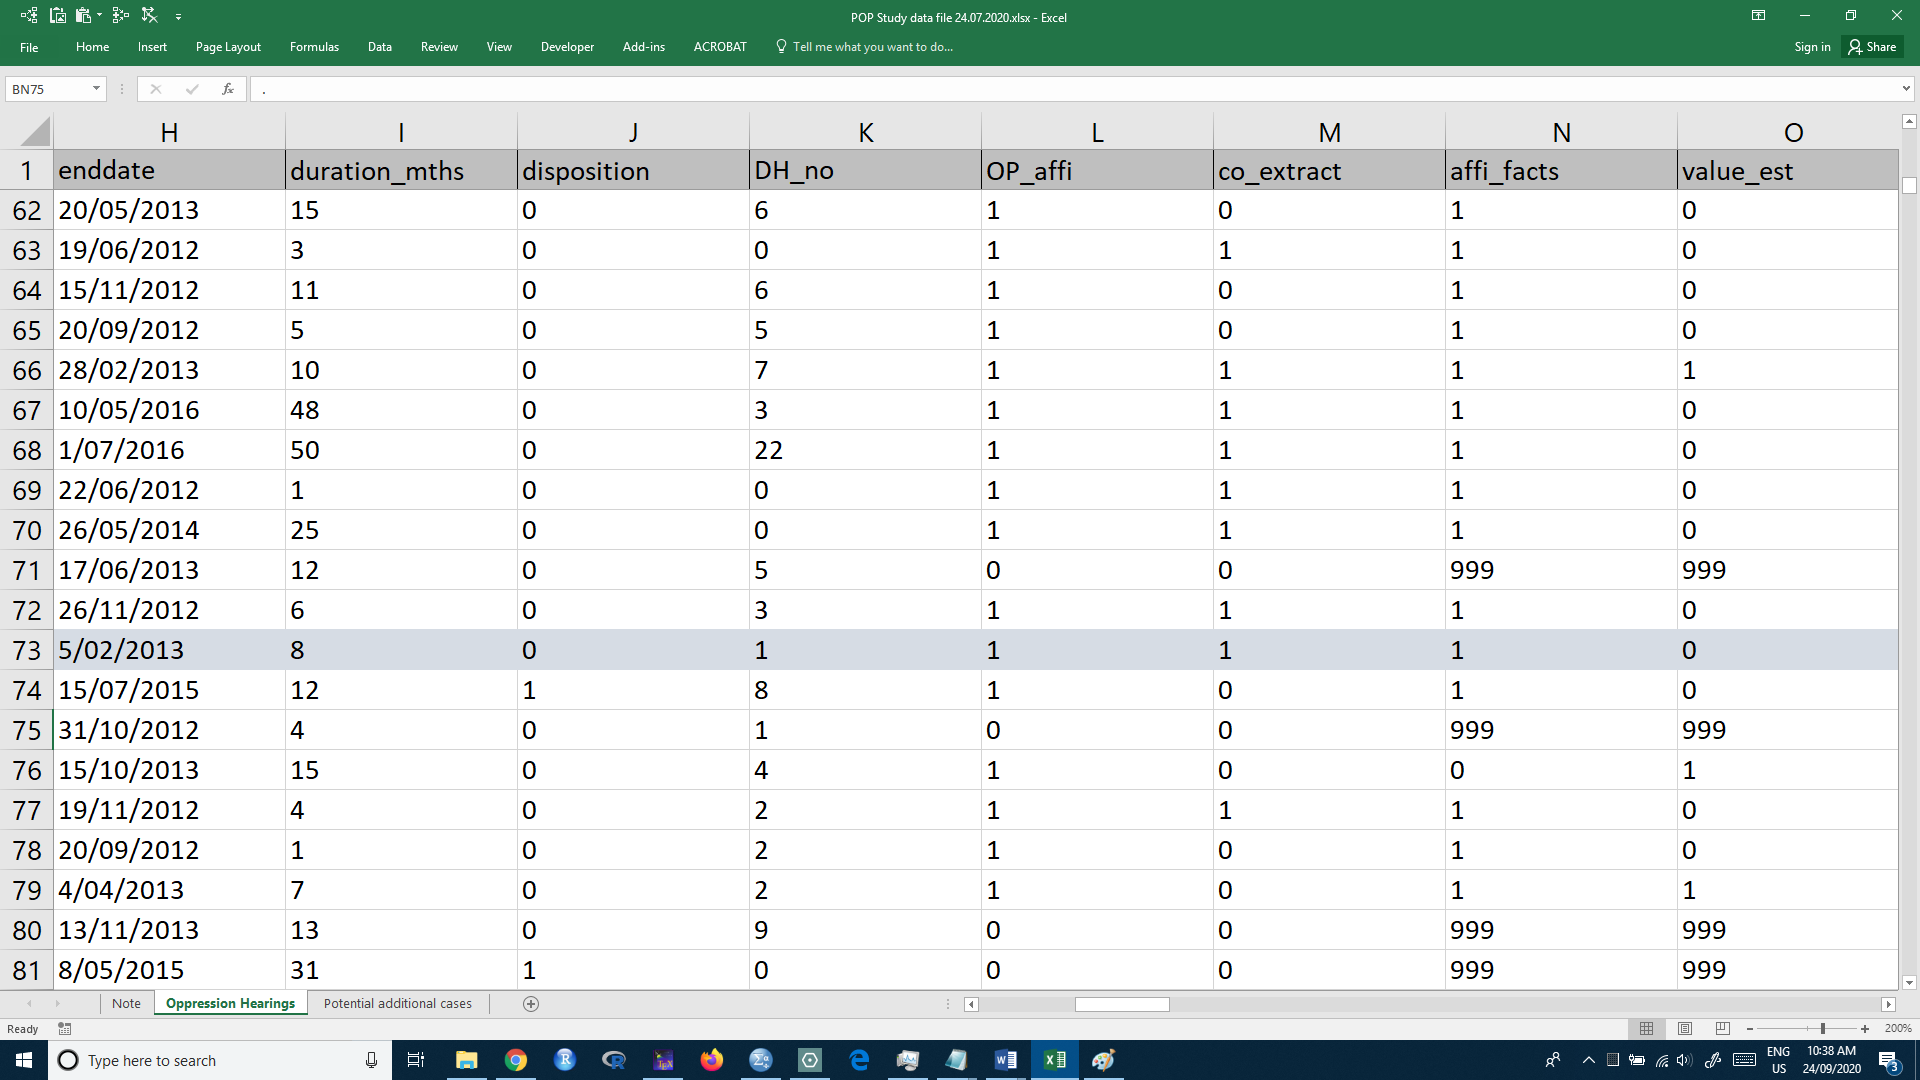
\includegraphics[width=.95\textwidth]{data/data_example_a.png}
		
	\end{frame}
	
	

	
	
	\section{Recognising good ideas}
	
	\begin{frame}{Modern context \citep[page 14]{spiegelhalter2019} }
		
		\centerfloat \centering	
		\includegraphics[width=.95\textwidth]{data/data-detective1.pdf}
		
	\end{frame}
	
	
	\begin{frame}{Ideas}
		
		\begin{itemize}
			\item<+-> Data summaries come before complex models.
			
			\item<+-> Lump and split dynamically.  
			
			\item<+-> Be flexible with ``data types''.
			
			\item<+-> Keep naming conventions simple and recognisable.
			
			\item<+-> Comment on any code and analysis steps that you take.
			
			\item<+-> Re-use your code and functions.
			
			\item<+-> Recognise that a plurality of systems may be useful.
			
			\item<+-> Investigate lots of models!
			
			\item<+-> Start with simple models and \text{then} add complexity.
			
			\item<+-> Test code to ensure you get the right answers.  
			\begin{itemize}
				\item Compare your R code with what you get in SPSS, for example.
				\item Use fake data or small subsets for testing.
			\end{itemize}
			
		\end{itemize}
	\end{frame}
	
	
	
	
	
	
	\section*{House keeping}
	
	
	\begin{frame}<100>{Lecture outcomes}
		\outcomes
	\end{frame}
	
	
	
	
	
	
	
	
	
	\begin{frame}[allowframebreaks]{Bibliography}
		\bibliographystyle{Chicago}
		\bibliography{data/ianBIBmaster}
	\end{frame}
	
\end{document}